\chapter{Matrices}

\index{matrix}

A \key{matrix} is a mathematical concept
that corresponds to a two-dimensional array
in programming. For example,
\[
A = 
 \begin{bmatrix}
  6 & 13 & 7 & 4 \\
  7 & 0 & 8 & 2 \\
  9 & 5 & 4 & 18 \\
 \end{bmatrix}
\]
is a matrix of size $3 \times 4$, i.e.,
it has 3 rows and 4 columns.
The notation $[i,j]$ refers to
the element in row $i$ and column $j$
in a matrix.
For example, in the above matrix,
$A[2,3]=8$ and $A[3,1]=9$.

\index{vector}

A special case of a matrix is a \key{vector}
that is a one-dimensional matrix of size $n \times 1$.
For example,
\[
V =
\begin{bmatrix}
4 \\
7 \\
5 \\
\end{bmatrix}
\]
is a vector that contains three elements.

\index{transpose}

The \key{transpose} $A^T$ of a matrix $A$
is obtained when the rows and columns in $A$
are swapped, i.e., $A^T[i,j]=A[j,i]$:
\[
A^T = 
 \begin{bmatrix}
  6 & 7 & 9 \\
  13 & 0 & 5 \\
  7 & 8 & 4 \\
  4 & 2 & 18 \\
 \end{bmatrix}
\]

\index{square matrix}

A matrix is a \key{square matrix} if it
has the same number of rows and columns.
For example, the following matrix is a
square matrix:

\[
S = 
 \begin{bmatrix}
  3 & 12 & 4  \\
  5 & 9 & 15  \\
  0 & 2 & 4 \\
 \end{bmatrix}
\]

\section{Operations}

The sum $A+B$ of matrices $A$ and $B$
is defined if the matrices are of the same size.
The result is a matrix where each element
is the sum of the corresponding elements
in $A$ and $B$.

For example,
\[
 \begin{bmatrix}
  6 & 1 & 4 \\
  3 & 9 & 2 \\
 \end{bmatrix}
+
 \begin{bmatrix}
  4 & 9 & 3 \\
  8 & 1 & 3 \\
 \end{bmatrix}
=
 \begin{bmatrix}
  6+4 & 1+9 & 4+3 \\
  3+8 & 9+1 & 2+3 \\
 \end{bmatrix}
=
 \begin{bmatrix}
  10 & 10 & 7 \\
  11 & 10 & 5 \\
 \end{bmatrix}.
\]

Multiplying a matrix $A$ by a value $x$ means
that each element of $A$ is multiplied by $x$.
For example,
\[
 2 \cdot \begin{bmatrix}
  6 & 1 & 4 \\
  3 & 9 & 2 \\
 \end{bmatrix}
=
 \begin{bmatrix}
  2 \cdot 6 & 2\cdot1 & 2\cdot4 \\
  2\cdot3 & 2\cdot9 & 2\cdot2 \\
 \end{bmatrix}
=
 \begin{bmatrix}
  12 & 2 & 8 \\
  6 & 18 & 4 \\
 \end{bmatrix}.
\]

\subsubsection{Matrix multiplication}

\index{matrix multiplication}

The product $AB$ of matrices $A$ and $B$
is defined if $A$ is of size $a \times n$
and $B$ is of size $n \times b$, i.e.,
the width of $A$ equals the height of $B$.
The result is a matrix of size $a \times b$
whose elements are calculated using the formula
\[
AB[i,j] = \sum_{k=1}^n A[i,k] \cdot B[k,j].
\]

The idea is that each element in $AB$
is a sum of products of elements in $A$ and $B$
according to the following picture:

\begin{center}
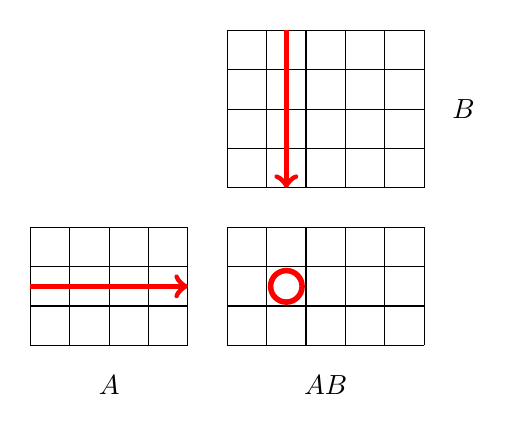
\begin{tikzpicture}[scale=0.5]
\draw (0,0) grid (4,3);
\draw (5,0) grid (10,3);
\draw (5,4) grid (10,8);

\node at (2,-1) {$A$};
\node at (7.5,-1) {$AB$};
\node at (11,6) {$B$};

\draw[thick,->,red,line width=2pt] (0,1.5) -- (4,1.5);
\draw[thick,->,red,line width=2pt] (6.5,8) -- (6.5,4);
\draw[thick,red,line width=2pt] (6.5,1.5) circle (0.4);
\end{tikzpicture}
\end{center}

For example,

\[
 \begin{bmatrix}
  1 & 4 \\
  3 & 9 \\
  8 & 6 \\
 \end{bmatrix}
\cdot
 \begin{bmatrix}
  1 & 6 \\
  2 & 9 \\
 \end{bmatrix}
=
 \begin{bmatrix}
  1 \cdot 1 + 4 \cdot 2 & 1 \cdot 6 + 4 \cdot 9 \\
  3 \cdot 1 + 9 \cdot 2 & 3 \cdot 6 + 9 \cdot 9 \\
  8 \cdot 1 + 6 \cdot 2 & 8 \cdot 6 + 6 \cdot 9 \\
 \end{bmatrix}
=
 \begin{bmatrix}
  9 & 42 \\
  21 & 99 \\
  20 & 102 \\
 \end{bmatrix}.
\]

Matrix multiplication is associative,
so $A(BC)=(AB)C$ holds,
but it is not commutative,
so $AB = BA$ does not usually hold.

\index{identity matrix}

An \key{identity matrix} is a square matrix
where each element on the diagonal is 1
and all other elements are 0.
For example, the following matrix
is the $3 \times 3$ identity matrix:
\[
 I = \begin{bmatrix}
  1 & 0 & 0 \\
  0 & 1 & 0 \\
  0 & 0 & 1 \\
 \end{bmatrix}
\]

\begin{samepage}
Multiplying a matrix by an identity matrix
does not change it. For example,
\[
 \begin{bmatrix}
  1 & 0 & 0 \\
  0 & 1 & 0 \\
  0 & 0 & 1 \\
 \end{bmatrix}
\cdot
 \begin{bmatrix}
  1 & 4 \\
  3 & 9 \\
  8 & 6 \\
 \end{bmatrix}
=
 \begin{bmatrix}
  1 & 4 \\
  3 & 9 \\
  8 & 6 \\
 \end{bmatrix} \hspace{10px} \textrm{and} \hspace{10px}
 \begin{bmatrix}
  1 & 4 \\
  3 & 9 \\
  8 & 6 \\
 \end{bmatrix}
\cdot
 \begin{bmatrix}
  1 & 0 \\
  0 & 1 \\
 \end{bmatrix}
=
 \begin{bmatrix}
  1 & 4 \\
  3 & 9 \\
  8 & 6 \\
 \end{bmatrix}.
\]
\end{samepage}

Using a straightforward algorithm,
we can calculate the product of
two $n \times n$ matrices
in $O(n^3)$ time.
There are also more efficient algorithms
for matrix multiplication\footnote{The first such
algorithm, with time complexity $O(n^{2.80735})$,
was published in 1969 \cite{str69}, and
the best current algorithm
works in $O(n^{2.37286})$ time \cite{gal14}.},
but they are mostly of theoretical interest
and such special algorithms are not needed
in competitive programming.


\subsubsection{Matrix power}

\index{matrix power}

The power $A^k$ of a matrix $A$ is defined
if $A$ is a square matrix.
The definition is based on matrix multiplication:
\[ A^k = \underbrace{A \cdot A \cdot A \cdots A}_{\textrm{$k$ times}} \]
For example,

\[
 \begin{bmatrix}
  2 & 5 \\
  1 & 4 \\
 \end{bmatrix}^3 =
 \begin{bmatrix}
  2 & 5 \\
  1 & 4 \\
 \end{bmatrix} \cdot
 \begin{bmatrix}
  2 & 5 \\
  1 & 4 \\
 \end{bmatrix} \cdot
 \begin{bmatrix}
  2 & 5 \\
  1 & 4 \\
 \end{bmatrix} =
 \begin{bmatrix}
  48 & 165 \\
  33 & 114 \\
 \end{bmatrix}.
\]
In addition, $A^0$ is an identity matrix. For example,
\[
 \begin{bmatrix}
  2 & 5 \\
  1 & 4 \\
 \end{bmatrix}^0 =
 \begin{bmatrix}
  1 & 0 \\
  0 & 1 \\
 \end{bmatrix}.
\]

The matrix $A^k$ can be efficiently calculated
in $O(n^3 \log k)$ time using the
algorithm in Chapter 21.2. For example,
\[
 \begin{bmatrix}
  2 & 5 \\
  1 & 4 \\
 \end{bmatrix}^8 =
 \begin{bmatrix}
  2 & 5 \\
  1 & 4 \\
 \end{bmatrix}^4 \cdot
 \begin{bmatrix}
  2 & 5 \\
  1 & 4 \\
 \end{bmatrix}^4.
\]

\subsubsection{Determinant}

\index{determinant}

The \key{determinant} $\det(A)$ of a matrix $A$
is defined if $A$ is a square matrix.
If $A$ is of size $1 \times 1$,
then $\det(A)=A[1,1]$.
The determinant of a larger matrix is
calculated recursively using the formula \index{cofactor}
\[\det(A)=\sum_{j=1}^n A[1,j] C[1,j],\]
where $C[i,j]$ is the \key{cofactor} of $A$
at $[i,j]$.
The cofactor is calculated using the formula
\[C[i,j] = (-1)^{i+j} \det(M[i,j]),\]
where $M[i,j]$ is obtained by removing
row $i$ and column $j$ from $A$.
Due to the coefficient $(-1)^{i+j}$ in the cofactor,
every other determinant is positive
and negative.
For example,
\[
\det(
 \begin{bmatrix}
  3 & 4 \\
  1 & 6 \\
 \end{bmatrix}
) = 3 \cdot 6 - 4 \cdot 1 = 14 
\]
and
\[
\det(
 \begin{bmatrix}
  2 & 4 & 3 \\
  5 & 1 & 6 \\
  7 & 2 & 4 \\
 \end{bmatrix}
) = 
2 \cdot
\det(
 \begin{bmatrix}
  1 & 6 \\
  2 & 4 \\
 \end{bmatrix}
)
-4 \cdot
\det(
 \begin{bmatrix}
  5 & 6 \\
  7 & 4 \\
 \end{bmatrix}
)
+3 \cdot
\det(
 \begin{bmatrix}
  5 & 1 \\
  7 & 2 \\
 \end{bmatrix}
) = 81.
\]

\index{inverse matrix}

The determinant of $A$ tells us
whether there is an \key{inverse matrix}
$A^{-1}$ such that $A \cdot A^{-1} = I$,
where $I$ is an identity matrix.
It turns out that $A^{-1}$ exists
exactly when $\det(A) \neq 0$,
and it can be calculated using the formula

\[A^{-1}[i,j] = \frac{C[j,i]}{det(A)}.\]

For example,

\[
\underbrace{
 \begin{bmatrix}
  2 & 4 & 3\\
  5 & 1 & 6\\
  7 & 2 & 4\\
 \end{bmatrix}
}_{A}
\cdot
\underbrace{
 \frac{1}{81}
 \begin{bmatrix}
   -8 & -10 & 21 \\
   22 & -13 & 3 \\
   3 & 24 & -18 \\
 \end{bmatrix}
}_{A^{-1}}
=
\underbrace{
 \begin{bmatrix}
  1 & 0 & 0 \\
  0 & 1 & 0 \\
  0 & 0 & 1 \\
 \end{bmatrix}
}_{I}.
\]

\section{Linear recurrences}

\index{linear recurrence}

A \key{linear recurrence}
can be represented as a function $f(n)$
such that the initial values are
$f(0),f(1),\ldots,f(k-1)$
and the larger values
are calculated recursively using the formula
\[f(n) = c_1 f(n-1) + c_2 f(n-2) + \ldots + c_k f (n-k),\]
where $c_1,c_2,\ldots,c_k$ are constant coefficients.

We can use dynamic programming to calculate
any value of $f(n)$ in $O(kn)$ time by calculating
all values of $f(0),f(1),\ldots,f(n)$ one after another.
However, if $k$ is small, it is possible to calculate
$f(n)$ much more efficiently in $O(k^3 \log n)$
time using matrix operations.

\subsubsection{Fibonacci numbers}

\index{Fibonacci number}

A simple example of a linear recurrence is the
following function that defines the Fibonacci numbers:
\[
\begin{array}{lcl}
f(0) & = & 0 \\
f(1) & = & 1 \\
f(n) & = & f(n-1)+f(n-2) \\
\end{array}
\]
In this case, $k=2$ and $c_1=c_2=1$.

\begin{samepage}
The idea is to represent the
Fibonacci formula as a
square matrix $X$ of size $2 \times 2$,
for which the following holds:
\[ X \cdot
 \begin{bmatrix}
  f(i) \\
  f(i+1) \\
 \end{bmatrix}
=
 \begin{bmatrix}
  f(i+1) \\
  f(i+2) \\
 \end{bmatrix}
 \]
Thus, values $f(i)$ and $f(i+1)$ are given as
''input'' for $X$,
and $X$ calculates values $f(i+1)$ and $f(i+2)$
from them.
It turns out that such a matrix is

\[ X = 
 \begin{bmatrix}
  0 & 1 \\
  1 & 1 \\
 \end{bmatrix}.
\]
\end{samepage}
\noindent
For example,
\[
 \begin{bmatrix}
  0 & 1 \\
  1 & 1 \\
 \end{bmatrix}
\cdot
 \begin{bmatrix}
  f(5) \\
  f(6) \\
 \end{bmatrix}
=
 \begin{bmatrix}
  0 & 1 \\
  1 & 1 \\
 \end{bmatrix}
\cdot
 \begin{bmatrix}
  5 \\
  8 \\
 \end{bmatrix}
=
 \begin{bmatrix}
  8 \\
  13 \\
 \end{bmatrix}
=
 \begin{bmatrix}
  f(6) \\
  f(7) \\
 \end{bmatrix}.
\]
Thus, we can calculate $f(n)$ using the formula
\[
 \begin{bmatrix}
  f(n) \\
  f(n+1) \\
 \end{bmatrix}
=
X^n \cdot
 \begin{bmatrix}
  f(0) \\
  f(1) \\
 \end{bmatrix}
=
 \begin{bmatrix}
  0 & 1 \\
  1 & 1 \\
 \end{bmatrix}^n
\cdot
 \begin{bmatrix}
  0 \\
  1 \\
 \end{bmatrix}.
\]
The value of $X^n$ can be calculated in
$O(k^3 \log n)$ time,
so the value of $f(n)$ can also be calculated
in $O(k^3 \log n)$ time.

\subsubsection{General case}

Let us now consider the general case where
$f(n)$ is any linear recurrence.
Again, our goal is to construct a matrix $X$
for which

\[ X \cdot
 \begin{bmatrix}
  f(i) \\
  f(i+1) \\
  \vdots \\
  f(i+k-1) \\
 \end{bmatrix}
=
 \begin{bmatrix}
  f(i+1) \\
  f(i+2) \\
  \vdots \\
  f(i+k) \\
 \end{bmatrix}.
\]
Such a matrix is
\[
X =
 \begin{bmatrix}
  0 & 1 & 0 & 0 & \cdots & 0 \\
  0 & 0 & 1 & 0 & \cdots & 0 \\
  0 & 0 & 0 & 1 & \cdots & 0 \\
  \vdots & \vdots & \vdots & \vdots & \ddots & \vdots \\
  0 & 0 & 0 & 0 & \cdots & 1 \\
  c_k & c_{k-1} & c_{k-2} & c_{k-3} & \cdots & c_1 \\
 \end{bmatrix}.
\]
In the first $k-1$ rows, each element is 0
except that one element is 1.
These rows replace $f(i)$ with $f(i+1)$,
$f(i+1)$ with $f(i+2)$, and so on.
The last row contains the coefficients of the recurrence
to calculate the new value $f(i+k)$.

\begin{samepage}
Now, $f(n)$ can be calculated in
$O(k^3 \log n)$ time using the formula
\[
 \begin{bmatrix}
  f(n) \\
  f(n+1) \\
  \vdots \\
  f(n+k-1) \\
 \end{bmatrix}
=
X^n \cdot
 \begin{bmatrix}
  f(0) \\
  f(1) \\
  \vdots \\
  f(k-1) \\
 \end{bmatrix}.
\]
\end{samepage}

\section{Graphs and matrices}

\subsubsection{Counting paths}

The powers of an adjacency matrix of a graph
have an interesting property.
When $V$ is an adjacency matrix of an unweighted graph,
the matrix $V^n$ contains the numbers of paths of
$n$ edges between the nodes in the graph.

For example, for the graph
\begin{center}
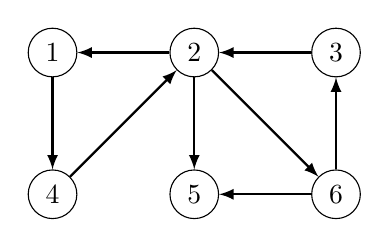
\begin{tikzpicture}[scale=0.9]
\node[draw, circle] (1) at (1,3) {$1$};
\node[draw, circle] (2) at (1,1) {$4$};
\node[draw, circle] (3) at (3,3) {$2$};
\node[draw, circle] (4) at (5,3) {$3$};
\node[draw, circle] (5) at (3,1) {$5$};
\node[draw, circle] (6) at (5,1) {$6$};

\path[draw,thick,->,>=latex] (1) -- (2);
\path[draw,thick,->,>=latex] (2) -- (3);
\path[draw,thick,->,>=latex] (3) -- (1);
\path[draw,thick,->,>=latex] (4) -- (3);
\path[draw,thick,->,>=latex] (3) -- (5);
\path[draw,thick,->,>=latex] (3) -- (6);
\path[draw,thick,->,>=latex] (6) -- (4);
\path[draw,thick,->,>=latex] (6) -- (5);
\end{tikzpicture}
\end{center}
the adjacency matrix is
\[
V= \begin{bmatrix}
  0 & 0 & 0 & 1 & 0 & 0 \\
  1 & 0 & 0 & 0 & 1 & 1 \\
  0 & 1 & 0 & 0 & 0 & 0 \\
  0 & 1 & 0 & 0 & 0 & 0 \\
  0 & 0 & 0 & 0 & 0 & 0 \\
  0 & 0 & 1 & 0 & 1 & 0 \\
 \end{bmatrix}.
\]
Now, for example, the matrix
\[
V^4= \begin{bmatrix}
  0 & 0 & 1 & 1 & 1 & 0 \\
  2 & 0 & 0 & 0 & 2 & 2 \\
  0 & 2 & 0 & 0 & 0 & 0 \\
  0 & 2 & 0 & 0 & 0 & 0 \\
  0 & 0 & 0 & 0 & 0 & 0 \\
  0 & 0 & 1 & 1 & 1 & 0 \\
 \end{bmatrix}
\]
contains the numbers of paths of 4 edges
between the nodes.
For example, $V^4[2,5]=2$,
because there are two paths of 4 edges
from node 2 to node 5:
$2 \rightarrow 1 \rightarrow 4 \rightarrow 2 \rightarrow 5$
and 
$2 \rightarrow 6 \rightarrow 3 \rightarrow 2 \rightarrow 5$.

\subsubsection{Shortest paths}

Using a similar idea in a weighted graph,
we can calculate for each pair of nodes the shortest
path between them that contains exactly $n$ edges.
To calculate this, we have to define matrix multiplication
in a new way, so that we do not calculate the numbers
of paths but minimize the lengths of paths.

\begin{samepage}
As an example, consider the following graph:
\begin{center}
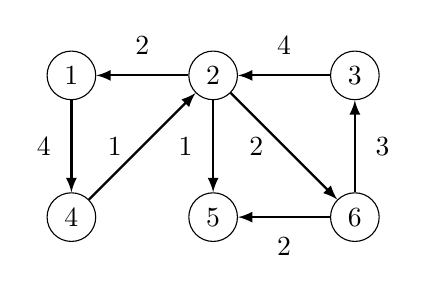
\begin{tikzpicture}[scale=0.9]
\node[draw, circle] (1) at (1,3) {$1$};
\node[draw, circle] (2) at (1,1) {$4$};
\node[draw, circle] (3) at (3,3) {$2$};
\node[draw, circle] (4) at (5,3) {$3$};
\node[draw, circle] (5) at (3,1) {$5$};
\node[draw, circle] (6) at (5,1) {$6$};

\path[draw,thick,->,>=latex] (1) -- node[font=\small,label=left:4] {} (2);
\path[draw,thick,->,>=latex] (2) -- node[font=\small,label=left:1] {} (3);
\path[draw,thick,->,>=latex] (3) -- node[font=\small,label=north:2] {} (1);
\path[draw,thick,->,>=latex] (4) -- node[font=\small,label=north:4] {} (3);
\path[draw,thick,->,>=latex] (3) -- node[font=\small,label=left:1] {} (5);
\path[draw,thick,->,>=latex] (3) -- node[font=\small,label=left:2] {} (6);
\path[draw,thick,->,>=latex] (6) -- node[font=\small,label=right:3] {} (4);
\path[draw,thick,->,>=latex] (6) -- node[font=\small,label=below:2] {} (5);
\end{tikzpicture}
\end{center}
\end{samepage}

Let us construct an adjacency matrix where
$\infty$ means that an edge does not exist,
and other values correspond to edge weights.
The matrix is
\[
V= \begin{bmatrix}
  \infty & \infty & \infty & 4 & \infty & \infty \\
  2 & \infty & \infty & \infty & 1 & 2 \\
  \infty & 4 & \infty & \infty & \infty & \infty \\
  \infty & 1 & \infty & \infty & \infty & \infty \\
  \infty & \infty & \infty & \infty & \infty & \infty \\
  \infty & \infty & 3 & \infty & 2 & \infty \\
 \end{bmatrix}.
\]

Instead of the formula
\[
AB[i,j] = \sum_{k=1}^n A[i,k] \cdot B[k,j]
\]
we now use the formula
\[
AB[i,j] = \min_{k=1}^n A[i,k] + B[k,j]
\]
for matrix multiplication, so we calculate
a minimum instead of a sum,
and a sum of elements instead of a product.
After this modification,
matrix powers correspond to
shortest paths in the graph.

For example, as
\[
V^4= \begin{bmatrix}
  \infty & \infty & 10 & 11 & 9 & \infty \\
  9 & \infty & \infty & \infty & 8 & 9 \\
  \infty & 11 & \infty & \infty & \infty & \infty \\
  \infty & 8 & \infty & \infty & \infty & \infty \\
  \infty & \infty & \infty & \infty & \infty & \infty \\
  \infty & \infty & 12 & 13 & 11 & \infty \\
 \end{bmatrix},
\]
we can conclude that the shortest path of 4 edges
from node 2 to node 5 has length 8.
This path is
$2 \rightarrow 1 \rightarrow 4 \rightarrow 2 \rightarrow 5$.

\subsubsection{Kirchhoff's theorem}

\index{Kirchhoff's theorem}
\index{spanning tree}

\key{Kirchhoff's theorem} provides a way
to calculate the number of spanning trees
of a graph as a determinant of a special matrix.
For example, the graph
\begin{center}
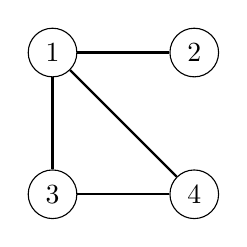
\begin{tikzpicture}[scale=0.9]
\node[draw, circle] (1) at (1,3) {$1$};
\node[draw, circle] (2) at (3,3) {$2$};
\node[draw, circle] (3) at (1,1) {$3$};
\node[draw, circle] (4) at (3,1) {$4$};

\path[draw,thick,-] (1) -- (2);
\path[draw,thick,-] (1) -- (3);
\path[draw,thick,-] (3) -- (4);
\path[draw,thick,-] (1) -- (4);
\end{tikzpicture}
\end{center}
has three spanning trees:
\begin{center}
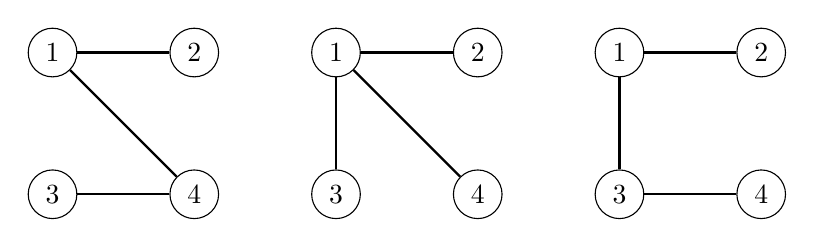
\begin{tikzpicture}[scale=0.9]
\node[draw, circle] (1a) at (1,3) {$1$};
\node[draw, circle] (2a) at (3,3) {$2$};
\node[draw, circle] (3a) at (1,1) {$3$};
\node[draw, circle] (4a) at (3,1) {$4$};

\path[draw,thick,-] (1a) -- (2a);
%\path[draw,thick,-] (1a) -- (3a);
\path[draw,thick,-] (3a) -- (4a);
\path[draw,thick,-] (1a) -- (4a);

\node[draw, circle] (1b) at (1+4,3) {$1$};
\node[draw, circle] (2b) at (3+4,3) {$2$};
\node[draw, circle] (3b) at (1+4,1) {$3$};
\node[draw, circle] (4b) at (3+4,1) {$4$};

\path[draw,thick,-] (1b) -- (2b);
\path[draw,thick,-] (1b) -- (3b);
%\path[draw,thick,-] (3b) -- (4b);
\path[draw,thick,-] (1b) -- (4b);

\node[draw, circle] (1c) at (1+8,3) {$1$};
\node[draw, circle] (2c) at (3+8,3) {$2$};
\node[draw, circle] (3c) at (1+8,1) {$3$};
\node[draw, circle] (4c) at (3+8,1) {$4$};

\path[draw,thick,-] (1c) -- (2c);
\path[draw,thick,-] (1c) -- (3c);
\path[draw,thick,-] (3c) -- (4c);
%\path[draw,thick,-] (1c) -- (4c);
\end{tikzpicture}
\end{center}
\index{Laplacean matrix}
To calculate the number of spanning trees,
we construct a \key{Laplacean matrix} $L$,
where $L[i,i]$ is the degree of node $i$
and $L[i,j]=-1$ if there is an edge between
nodes $i$ and $j$, and otherwise $L[i,j]=0$.
The Laplacean matrix for the above graph is as follows:
\[
L= \begin{bmatrix}
  3 & -1 & -1 & -1 \\
  -1 & 1 & 0 & 0 \\
  -1 & 0 & 2 & -1 \\
  -1 & 0 & -1 & 2 \\
 \end{bmatrix}
\]

The number of spanning trees equals
the determinant of a matrix that is obtained
when we remove any row and any column from $L$.
For example, if we remove the first row
and column, the result is

\[ \det(
\begin{bmatrix}
  1 & 0 & 0 \\
  0 & 2 & -1 \\
  0 & -1 & 2 \\
 \end{bmatrix}
) =3.\]
The determinant is always the same,
regardless of which row and column we remove from $L$.

Note that a special case of Kirchhoff's theorem
is Cayley's formula in Chapter 22.5,
because in a complete graph of $n$ nodes

\[ \det(
\begin{bmatrix}
  n-1 & -1 & \cdots & -1 \\
  -1 & n-1 & \cdots & -1 \\
  \vdots & \vdots & \ddots & \vdots \\
  -1 & -1 & \cdots & n-1 \\
 \end{bmatrix}
) =n^{n-2}.\]



